\newcommand{\Placeholder}[1]{$\langle\!\langle\mbox{\textrm{#1}}\rangle\!\rangle$}
\newcommand{\bfn}[1]{\textup{#1}}
\newcommand{\Src}[1]{\texttt{#1}}
\newcommand{\fn}[1]{\mathit{#1}}
\newcommand{\modify}[3]{{\underline{\sf{#1}}:} {\color{blue}{#2}} {\color{green}{\mbox{$\Rightarrow$}}} {\color{red}{#3}}}
\newcommand{\todo}[2]{{\underline{\textsf{#1}}:} {\color{red}{$\spadesuit$#2$\spadesuit$}}}
\newcommand{\hack}{{\color{red}{$\blacklozenge$}}}


\chapter{Parallelization Of XPath Queries on Top of BaseX}

On the topic of parallelelization of XPath queires, one practical and promising
approach was proposed by Bordawekar et al.~\cite{Bord10} in 2009. In this study,
three partitioning strategies were presented, i.e. data partitioning, query
partitiooning  and hybrid partitioing startegies,  making it possible to
parallelize XPath queries by partitioning an XPath query into subqueries and
evaluating them in parallel on XML trees.

However, since this study was based on an XSLT processing, it is thus not clear
to the following questions: \textit{(1) Whether and how can we apply their
partitioning strategies to XML database engines? (2) What speedup can we achieve
on large XML documents?}.

To answer the above two questions, we introduce our implementations on top of a
state-of-the-art XML database engine BaseX with two large XML documents sized 
1.1 GB and 1.85 GB by reviving and extending Bordawekar et al's study. We propose
three implementations on the base of the original idea from the paper and we also
extended our implementations in term of BaseX by exploiting its optimizations.
We experimentally demonstrate the performance on top of BaseX with two large 
XML documents. The experiment results proved that it is
possible to obtain significant speedups by simply rewriting queries into
subqueries and parallelizing the evaluation of them on top of an XML database
engine over gigabytes of XML documents, without need to modify source code of the engine.

%\input{basex/partitions}

\section{BaseX: An XML Database Engine}
\label{sect:basex}

To begin with, we give a brief introduction to BaseX, which is both a
state-of-the-art XML database and an XQuery/XPath 3.1 processor (refer to the
official documentation~\cite{basex864} for more details). BaesX provides
significant features in processing XML data sets. The following are the BaseX's
features particularly important for our study:

\begin{itemize}
	\item Full support of XQuery 3.1, especially arrays and XQuery Update Facility;
	\item XQuery extension for database operations, especially index-based
	random access;
	\item XQuery extension for full-text operations, especially
	\Src{ft:tokenize};
	\item Support of in-memory XML databases;
	\item Query optimization based on various indices.
	\item Support of concurrent transactions in the server mode.
\end{itemize}

The first three are concerned with the expressiveness of queries and the rests
are concerned with performance.

The most important (practically essential) feature to our implementations is
index-based random access to nodes of an XML database in BaseX. BaseX offers
indices that enable us to access any node in constant time. The PRE index, which
denotes the position of a node in the document order, brings the fastest
constant-time access in BaseX. Function \Src{db:node-pre} returns the PRE value
of a given node and function \Src{db:open-pre} returns the node of a given PRE
value. For example, given a BaseX database ``exampledb'', as shown below.
\begin{lstlisting}[escapechar=\@]
@$^1$@<books>
  @$^2$@<book>
	 @$^3$@<name>@$^4$@XML</name>
	 @$^5$@<author>@$^6$@Jack</author>
  @$^{\phantom{3}}$@</book>
@$^{\phantom{1}}$@</books>@\textrm{~,}@
\end{lstlisting}
where a left superscript denotes a PRE value. Now, consider the following query.
\begin{lstlisting}
for $node in db:open(``exampledb'')/books/book
return db:node-pre($node)
\end{lstlisting}
The querys selects \texttt{book} in `exampledb' and the result of \texttt{\$node} is
\verb|<book>...</book>|. Then, after applying the \texttt{db:node-pre} function
the final result is 2. PRE values are well-suited for representing intermediate
results of XPath queries because a PRE value is merely an integer that makes it
efficient to restart a tree traversal with PRE values. Letting a PRE value be 2
on the `exampledb', we use the following query as an example.

\begin{lstlisting}
for $pre in db:open-pre(``exampledb'', 2)/author
return $node
\end{lstlisting}

The \texttt{db:open-pre} takes the database and PRE as arguments to locate the
\texttt{book} node. Then it selects the \texttt{author} of \texttt{book}. The final
result is \verb|<author>Jack</author>|.


Arrays are useful for efficiently implementing block partitioning. On BaseX, the
length of an array is returned in constant time and the subarray of a specified
range is extracted in logarithmic time\footnote{In fact, both sequences and
arrays on BaseX are implemented with finger trees and therefore the
corresponding operations on sequences have the same cost.}. XQuery Update
Facility over in-memory databases strongly supports efficient use of temporary
databases for holding results of queries. Function \Src{ft:tokenize}, which
tokenizes a given string to a sequence of token strings, can implement
deserialization of sequences/arrays efficiently.  

BaseX's query optimization is so powerful that it is not unusual to improve time
complexity. For example, path index enables pruning
traversal of descendants and attribute index enables instant access to
the nodes that have a specific attribute name or value. With aggressive constant
propagation, BaseX exploits most constants including database metadata and PRE
values found in a given query for query optimization. Prevention of spoiling it,
as to be described in Section~\ref{sect:opt}, is therefore of crucial importance
for performance.

Lastly, BaseX can work in a client-server mode. A BaseX server can handle
concurrent transactions requested from BaseX clients with multiple threads
depending on the server's configurations. Read transactions that do not modify
data, such as XPath queries, are executed in parallel without waiting or using
locks in BaseX.


\section{Implementing Data Partitioning with BaseX}
\label{sect:dpsimpl}

In this section, we describe our two implementations for data partitioning
strategy, namely the client-side implementation and the server-side
implementation, on top of BaseX.

Data partitioning is to split a given query into a prefix query and a suffix
query, e.g., from \texttt{$q_1$/$q_2$} to prefix $q_1$ and suffix $q_2$, and to
run the suffix query in parallel on each node of the result of the prefix query.
The results of suffix queries are concatenated in document order to form the 
final result.


Our implementations are Java programs that involve a BaseX client. They
spawn $P$ threads (usually P is no more than the number of physical cores) and 
create a connection to a BaseX server for each thread so
as to run multiple queries in parallel after a prefix query. Merging $P$ partial
results in the form of string is sequentially implemented. The main difference
between the client-side and the server-side implementations is the way how the results of prefix
queries are handled. In the rest of this section, we describe them by using
XM3(a) shown in Table~\ref{tab:dpsqueries} as a running example, assuming input
database to be named \Src{`xmark.xml'}.

\subsection{Client-side Implementation}

The client-side implementation is a simple implementation of data partitioning
strategy with database operations on BaseX. It sends the server a prefix query 
to be executed and the PRE values of matched nodes are returned. The
following XQuery expression is used for the prefix query of XM3(a).

\begin{lstlisting}
for $x in db:open(``xmark'')/site//open_auction
return db:node-pre($x)
\end{lstlisting}

Let this prefix query return sequence \Src{(2, 5, 42, 81, 109, 203)}. 
Letting $P = 3$, it is block-partitioned to \Src{(2, 5)}, \Src{(42,
81)}, and \Src{(109, 203)}, each of which is assigned to a thread. To avoid
repetitive ping-pong between a client and the server, we use the following
suffix query template:

\vspace{10mm}
\begin{lstlisting}[escapechar=\@]
for $x in @\Placeholder{sequence of PRE}@
return db:open-pre(``xmark'', $x)/bidder[last()]@\textrm{~,}@
\end{lstlisting}
where \Placeholder{sequence of PRE} is a placeholder to be replaced with a
concrete partition, e.g., \Src{(42, 81)}. Each thread instantiates this template
with its own partition and sends the server the instantiated query.


\subsection{Server-side Implementation}

A necessary task on the results of a prefix query is to block-partition them.
The client-side implementation simply processes it on the client side. In fact,
we can also implement it efficiently on the server side by utilizing BaseX's
features.

First, we prepare an in-memory database named \Src{``tmp''} and initialized with
\Src{<root> </root>}, which is a temporary database for storing the results of a
prefix query.  The prefix query is \texttt{/site//open\_auction} and it selects 
all \texttt{open\_auction} and return the PRE values of matched nodes. 
It is implemented as follows:

\begin{lstlisting}[escapechar=\@]
let $P := @\Placeholder{number of partitions}@
let $arr := array { for $x in db:open(``xmark'')/site//open_auction
                       db:node-pre($x) }
for $i in 1 to $P
return insert node element part { $block_part($i, $P, $arr) }
         as last into db:open('tmp')/root@\textrm{~,}@
\end{lstlisting}
where \Placeholder{number of partitions} denotes a placeholder to be replaced
with a concrete value of $P$ and \verb|$block_part($i, $P, $arr)| denotes the
\verb|$i|-th subarray of \verb|$P|-block partitioned \verb|$arr|. With the array
operations of extracting length and subarray, \verb|$block_part| is implemented
in logarithmic time.

In the example case used earlier, \Src{``tmp''} database results in the following:
\newpage
\begin{lstlisting}[escapechar=\@]
@$^1$@<root>
  @$^2$@<part>@$^3$@2 5</part>@$^4$@<part>@$^5$@42 81</part>@$^6$@<part>@$^7$@109 203</part>
@$^{\phantom{1}}$@</root>@\textrm{~,}@
\end{lstlisting}
where a left superscript denotes a PRE value. Note that its document structure
determines the PRE value of $i$th partition to be $2i+1$.

A suffix query is implemented with deserialization of a partition as follows:
\begin{lstlisting}[escapechar=\@]
for $x in ft:tokenize(db:open-pre(``tmp'', @\Placeholder{PRE of partition}@))
return db:open-pre('xmark', xs:integer($x))/bidder[last()])@\textrm{~,}@
\end{lstlisting}
where \Placeholder{PRE of partition} denotes a placeholder to be replaced with
the PRE value of a target partition.

In most case, the server-side implementation is more efficient because communication data
between clients and a server except for output is reduced to a constant size.


\begin{figure}[tbp]
	\centering
	\caption{List of XPath queries and their partitioning, where pre and suf
		mean prefix query and suffix query respectively}
	\label{tab:dpsqueries}
	\small
	\begin{tabular}{l|l}
		\hline
		Key & Query \\
		\hline
		XM1  & \verb|/site//*[name(.)="emailaddress" or name(.)="annotation" or| \\
		& \verb| name(.)="description"] |\\
		XM1(a) & pre = \verb|/site/*|, \\
		& suf = \verb|descendant-or-self::*[name(.)="emailaddress" or | \\
		& \verb|     name(.)="annotation" or name(.)="description"]| \\
		\hline
		XM2 & \verb|/site//incategory[./@category="category52"]/parent::item/@id| \\
		XM2(a) & pre = \verb|/site//incategory|, \quad \\
		& suf = \verb|self::*[./@category="category52"]/parent::item/@id| \\
		XM2(b) & pre = \verb|/site/*|, \quad  \\
		& suf = \verb|descendant-or-self::incategory[./@category="category52"]|\\
		& \verb|      /parent::item/@id| \\
		XM2(c) & pre = \verb|db:attribute("xmark10", "category52")|, \\
		& suf = \verb|parent::incategory[ancestor::site/parent::document-node()]| \\
		& \verb|      /parent::item/@id| \\
		\hline
		XM3 & \verb|/site//open_auction/bidder[last()]| \\
		XM3(a) & pre = \verb|/site//open_auction|, \quad suf = \verb|bidder[last()]| \\
		XM3(b) & pre = \verb|/site/*|, \quad \\
		& suf = \verb|descendant-or-self::open_auction/bidder[last()]| \\
		XM3(c) & pre = \verb|/site/open_auctions/open_auction|, \quad suf = \verb|bidder[last()]| \\
		\hline
		XM4 & \verb|/site/regions/*/item[./location="United States" and ./quantity > 0| \\
		& \verb| and ./payment="Creditcard" and ./description and ./name]| \\
		XM4(a) & pre = \verb|/site/regions/*|, \quad\\
		& suf = \verb|item[./location="United States" and ./quantity > 0 and | \\
		& \verb|     ./payment="Creditcard" and ./description and ./name]| \\
		XM4(b) & pre = \verb|/site/regions/*/item|, \quad \\
		& suf = \verb|self::*[./location="United States" and ./quantity > 0 and|  \\
		& \verb|     ./payment="Creditcard" and ./description and ./name]| \\
		XM4(c) & pre = \verb|db:text("xmark10", "Creditcard")/parent::payment|, \\
		& suf = \verb|parent::item[parent::*/parent::regions| \\
		& \verb|      /parent::site/parent::document-node()]| \\
		& \verb|     [location = "United States"][0.0 < quantity][description][name]| \\
		\hline
		XM5 & \verb|/site/open_auctions/open_auction/bidder/increase| \\
		XM5(a) & pre = \verb|/site/open_auctions/open_auction/bidder|, \quad suf = \verb|increase| \\
		XM5(b) & pre = \verb|/site/open_auctions/open_auction|, \quad suf = \verb|bidder/increase| \\
		\hline
		XM6 & \verb|/site/regions/*[name(.)="africa" or name(.)="asia"]| \\
		&  \verb|/item/description/parlist/listitem| \\
		XM6(a) & pre = \verb|/site/regions/*|, \quad \\
		& suf = \verb|self::*[name(.)="africa" or name(.)="asia"]|\\
		& \verb|     /item/description/parlist/listitem| \\
		XM6(b) & pre = \verb|/site/regions/*[name(.)="africa" or name(.)="asia"]/item|, \quad  \\
		& suf = \verb|description/parlist/listitem| \\
		\hline
		DBLP1 & \verb|/dblp/article/author|\\
		DBLP1(a) & pre = \verb|/dblp/article|,   suf = \verb|author|\\
		\hline
		DBLP2 & \verb|/dblp//title|\\
		DBLP2(a) & pre = \verb|/dblp/*|,  suf = \verb|self::*//title|\\
		\hline
	\end{tabular}
\end{figure}


\section{Implementing Query Partitioning with BaseX}
\label{sect:qpsimpl}

In this section, we describe our implementation of query partitioning strategy on top of
BaseX. The implementation of query partitioning strategy is also a Java program that
involves a BaseX client. This implementation
is relatively simpler than that for data partitioning.  It has two-phase, 
a parallel evaluating phase and a merge phase.  In the
parallel evaluating phase, a query is divided into multiple subqueries, which 
are executed by a BaseX server in parallel. In the second phase,
the results of all subquery are merged together into a whole as the final
result. In the following paragraphs, we focus the parallel evaluating phase 
of query partitioning in detail.


There are two ways of partitioning an XPath query in the
parallel evaluating phase: position-based partitioning and predicate-based
partitioning. Position-based partitioning is to divide the query by the
\texttt{position} function on a specific location step.  It is based on the
partition of children of a node in particular positions such that these children
are divided into multiple groups in order. Then, we evaluate on these groups of
nodes and its branches in parallel. Let us take XM5 as example. The children
nodes of \texttt{/site/open\_auctions} on `xmark10.xml' is 120000. Letting P =
3, then we can use the \texttt{position} function to divide the query into three
subqueries as follows:\\
\begin{small}
	\verb|/site/open_auctions\open_auction[position()=1 to 40000]\bidder/increase|\\
	\verb|/site/open_auctions\open_auction[position()=40001 to 80000]\bidder/increase|\\
	\verb|/site/open_auctions\open_auction[position()=80001 to 120000]\bidder/increase|\\
\end{small}
These three subqueries cover exactly the same parts on the target XML document 
as that of the original query and returns in turn the same results. 
Node that since the query is divided
by the \texttt{position} function in document order, the results are also in
document order. Thus, we can simply merge the results orderly to form the final
result.

% branch-based partitioning

As for the predicate-based partitioning, it is not promising to be introduced in
term of XML database engines. This is because it takes extra time to
merge the results of subqueries. For example, given a query \texttt{/q1[q2 or
	q3]} that is divided into \texttt{q1[q2]} and \texttt{q1[q3]}, we can retrieve
results from both queries. Since the operation is an `\texttt{or}', we need to
perform an ordered union to the results of the two subqueries. However, since
the resultant nodes in the results, there are two difficulties to merge them.
First, we need to determine the order of nodes in the results. Second, the
merging process itself is time-consuming when the results are in plain text.
Therefore, we do not discuss this partitioning in our study.

We also extend the query partitioning strategy by partitioning the children with
different names, called branch-based partitioning. We exploit the structure of the
input XML document to evaluate subqueries on the branches of a node by walking
through its children in parallel. Let us take XM1(d) on `\texttt{xmark10.xml}'
as an example. Since the root of the document has only six nodes:
\texttt{regions}, 
\texttt{categories}, 
\texttt{catgraph}, 
\texttt{people},
\texttt{open\_auctions},
\texttt{closed\_auctions}, 
we can make the input query into six corresponding sub
queries. Given the first child \texttt{regions} of the root, we make the
corresponding subquery as
\verb|/site/regions/descendant-or-self::incategory.../@id|, which is to be
evaluated through only the first branch of the root  and selects \texttt{@id}s
that matches the query in that branch. 
The six corresponding sub queries cover exactly the same part of the
original query and return the same results. Because the children of the root are
in document order, the results are also ordered as long as the results are
merged in the same order.


\begin{figure}[tbp]
	\centering
	\caption{List of XPath queries used for query partitioning, where [pos] denotes position-based partitioning and \{name\} denotes branch-based partitioning.}
	\label{tab:qpsqueries}
	\small
	\begin{tabular}{l|l}
		\hline
		XM1 & \verb|/site//*[name(.)="emailaddress" or name(.)="annotation"| \\
		& \verb| or name(.)="description"]|\\
		XM1(d) & \verb|/site/*[pos]/descendant-or-self::*[name(.)="emailaddress" |\\
		&  or name(.)="annotation" or name(.)="description"]| \\
		XM1(e) & \verb|/site/{name}/descendant-or-self::*[name(.)="emailaddress" |\\
		& \verb| or name(.)="annotation" or name(.)="description"]|\\
		\hline
		XM2 & \verb|/site//incategory[./@category="category52"]/parent::item/@id| \\
		XM2(d) & \verb|/site/regions/*[pos]/item/incategory[./@category="category52"]|\\
		& \verb|/parent| \\
		XM2(e) & \verb|/site/regions/{name}/item/incategory[./@category="category52"]|\\
		& \verb|/parent| \\
		\hline
		XM3 & \verb|/site//open_auction/bidder[last()]|\\
		XM3(d) & \verb|/site/open_auctions/open_auction[pos]/bidder[last()]|\\
		\hline
		XM4 & \verb|/site/regions/*/item[./location="United States" and ./quantity| \\
		& \verb| > 0 and ./payment="Creditcard"and ./description and ./name]|\\
		XM4(d) & \verb|/site/regions/*[pos]/item[./location="United States"|\\
		& \verb|and ./quantity > 0 and ./payment="Creditcard and ./description| \\
		& \verb|and ./name]| \\
		XM4(e) & \verb|/site/regions/{name}/item[./location="United States"|\\
		& \verb|and ./quantity > 0 and ./payment="Creditcard" and ]|\\
		& \verb|./description and ./name| \\
		\hline
		XM5 & \verb|/site/open_auctions/open_auction/bidder/increase| \\
		XM5(d) & \verb|/site/open_auctions/open_auction[pos]/bidder/increase|\\
		\hline
		XM5(e) & \verb|/site/open_auctions/open_auction/bidder[pos]/increase|\\
		\hline
		XM6 & \verb|/site/regions/*[name(.)="africa" or name(.)="asia"]| \\
		& \verb|/item/description/parlist/listitem| \\
		XM6(d) & \verb|/site/regions/*[pos][name(.)="africa" or name(.)="asia"]| \\
		& \verb|/item/description/parlist/listitem| \\
		XM6(e) & \verb|/site/regions/\{name\}[name(.)="africa" or name(.)="asia"]| \\
		& \verb|/item/description/parlist/listitem| \\
		\hline
		DBLP1 & \verb|/dblp/article/author| \\
		DBLP1(d) & \verb|/site/regions/*[pos][name(.)="africa" or name(.)="asia"]| \\
		& \verb|/item/description/parlist/listitem|\\
		\hline
		DBLP2 & \verb|/dblp//title| \\
		DBLP2(d) & \verb|/dblp/{name}/titlem|\\
		\hline
	\end{tabular}
\end{figure}


%In query partitioning, the position-based and branch-based partitions 
%in our study are the same, which evaluate a
%query through dividing the children of a node. There, however, still are three
%main differences between them. First, position-based partitioning is not
%sensitive to the number of children of a node, i.e. no matter how big or small
%the number of nodes is, it is always available in both cases. This is because
%the \texttt{position} function can process a range of nodes in a subquery. As
%for branch-based partitioning, it is usually feasible only in case when the
%number of children is small. This is because each child makes a sub query. Thus,
%when the number of children is too big, there are by too many subqueries and
%need too many threads that may excess the number of available threads. In
%additional, the overhead of parsing theses subqueries is dramatic. Third, the
%branch-based is more  likely to be limited to the structure of input XML
%document. This is because  in real world XML documents, it is more likely to be
%ill-balanced when the names  of children of a node are different.  


\section{Integration with Query Optimization}
\label{sect:opt}

As mentioned in Section~\ref{sect:basex}, BaseX is equipped with a powerful
query optimizer. Some queries can be optimized to reduce execute time. For
example, BaseX optimizes XM3 can be optimized as follows.

\begin{lstlisting}
/site/open_auctions/open_auction/bidder[last()]
\end{lstlisting}

This optimization is on the basis of the path index, which brings knowledge that
\Src{open\_auction} exists only immediately below \Src{open\_auctions} and
\Src{open\_auctions} exists only immediately below \Src{site}. Because a step of
descendant-or-self axis (\Src{//open\_auction}) is replaced with two steps of
child axes (\Src{/open\_auctions/open\_auction}), the search space of this query
has been significantly reduced. Note that a more drastic result is observed in
XM2, where the attribute index is exploited through function \Src{db:attribute}. 

Partitioning strategies convert a given query to two separate ones and therefore
affects the capability of BaseX in query optimization. In fact, the suffix query
of XM3(b) is not optimized to the corresponding part of optimized XM3 because
BaseX does not utilize indices for optimizing queries starting from nodes
specified with PRE values even if possible in principle. Most index-based
optimizations are limited to queries starting from the document root. This is a
reasonable design choice in query optimization because it is expensive to check
all PRE values obtained from the evaluation of a prefix query. However, we do
not have to check all PRE values that specify the starting nodes of the suffix
query because of the nature of data partitioning, of which BaseX is unaware.
This discord between BaseX's query optimization and data partitioning may incur
serious performance degradation, and it also occurs in query partitioning
strategy in term of parallelizing subquereis.

A simple way of resolving this discord is to apply partitioning strategies to
the suffix queries after BaseX's query optimization. Partitioning strategies are
applicable to any multi-step XPath query in principle. Even if an optimized
query is thoroughly different from its original query as in XM2, it is entirely
adequate to apply both partitioning strategies to the optimized query,
forgetting the original. In fact, XM2--4(c) are instances of such data
partitioning after optimization.

The simplicity of this coordination brings two big benefits. One is that we are
still able to implement partitioning strategies only by using BaseX's dumps of
optimized queries without any modification on BaseX. The other is that it is
very easy to implement partitioning strategies into compilation in BaseX; we can
just add a data/query-partitioning pass after all existing query optimization
passes without any interference.


\def \t#1{t$_#1$}

\section{Experiments and Evaluations}
\label{sect:exper}

In this section, we introduce the experiments conducted on two datasets for
evaluating the performance of our implementations. We report the experiment
results and present our observations and perceptives based on the results.





% --------------------------------------------------
\subsection{Experimental Setting}

We have conducted several experiments to evaluate the performance of our
implementations of parallel XPath queries. All the experiments were conducted on
a computer that equipped with two Intel Xeon E5-2620 v3 CPUs (6 cores, 2.4GHz,
Hyper-Threading off) and 32-GB memory (DDR4-1866). Software we used ware Java
OpenJDK ver. 9-internal (64-Bit Server VM) and BaseX ver. 8.6.4 with minor
modifications to enable TCP\textunderscore NODELAY, which is
used to improve tcp/ip networks and decrease the number of packets.

We used two larege XML documents for the experiments: \texttt{xmark10.xml} and
\texttt{dblp.xml}. The dataset \texttt{xmark10.xml} is an XMark
dataset~\cite{XMark} generated with the parameter 10, which was of 1.1 GB and
had 16 million nodes. The root of the XMark tree has six children
\verb|regions|, \verb|people|, \verb|open_auctions|, \verb|closed_auctions|,
\verb|catgraph|, and \verb|categories|, which have 6, 255000, 120000, 97500,
10000, and 10000 children, respectively. The dataset \texttt{dblp.xml} was
downloaded on Febrary 13, 2017 from~\cite{DBLP}, which is an open bibliographic
information database on major computer science journals and proceedings. It
sizes 1.85 GB and has 46 million nodes. The root has 5.5 million nodes of eight
different names, including  \texttt{article},  \texttt{book},
\texttt{incollections},  \texttt{inproceedings},  \texttt{masterthesis},
\texttt{phdthesis}, \texttt{proceedings},  \texttt{www}.


We used the XPath queries shown in Table~\ref{tab:dpsqueries} for data
partitioning and Table~\ref{tab:qpsqueries} for query partitioning, which are
the same as those used in~\cite{BoLS09}, and measured execution times until we
obtained the whole serialized string as the result. The execution time does not
include the loading time, that is, the input XML tree was loaded into memory
before the execution of queries. To reduce the effect of fluctuations, we
measured execution time for 51 times, and calculated their average after
removing top-10 and bottom-10 results.


% --------------------------------------------------
\subsection{Evaluation on Implementations of Data Partitioning Strategy}

In this section, we evaluate two of our implementations of data partitioning
strategy. We also analysis the speedup and scalability of them.

\subsubsection{Total Execution Time}

\begin{table}[tbp]
\caption{Summary of execution time of data partitioning}
\label{Table:summary}
\small
\setlength{\doublerulesep}{.4pt}
\centering\begin{tabular}{l|c|rr@{~(}r@{)}|rr@{~(}r@{)}|rr}
\hline \hline
~~Key & orig $t_o$~ & \multicolumn{3}{c|}{client-side} & \multicolumn{3}{c|}{server-side} & \multicolumn{2}{c}{Result size} \\
	&       			& seq $t_s$~   	& par $t_p$~   	& $t_o/t_p$	& seq $t_s$~	& par $t_p$~	& $t_o/t_p$	& prefix~	& final~ \\
\hline
XM1(a)	& 25796.64			& 27916.83	& 12392.80	& 2.08		& 28161.89	& 11484.99	& 2.25		& 54		& 994 M \\
\hline
XM2(a)	& \multirow{3}{*}{1.33}		& 2996.85	& 959.18	& 0.00		& 1159.78	& 760.62	& 0.00		& 6.62 M	& \multirow{3}{*}{1.55 K} \\
XM2(b)	&				& 1018.59	& 707.38	& 0.00		& 894.94	& 529.75	& 0.00		& 54		&  \\
XM2(c)	&				& 3.43		& 4.56		& 0.29		& 5.29		& 6.26		& 0.21		& 671		&  \\
\hline
XM3(a)	& \multirow{3}{*}{595.75}	& 900.69	& 297.88	& 2.00		& 706.95	& 226.54	& 2.63		& 1.08 M	& \multirow{3}{*}{14.5 M} \\
XM3(b)	&				& 1519.92	& 1148.42	& 0.52		& 1472.53	& 987.48	& 0.60		& 54		&  \\
XM3(c)	&				& 1029.85	& 308.67	& 1.93		& 723.44	& 297.31	& 2.00		& 1.08 M	&  \\
\hline
XM4(a)	& \multirow{3}{*}{798.16}	& 1290.36	& 699.99	& 1.14		& 1241.34	& 559.32	& 1.43		& 49		& \multirow{3}{*}{26.4 M} \\
XM4(b)	&				& 1786.89	& 564.82	& 1.41		& 1216.57	& 406.93	& 1.96		& 1.75 M	&  \\
XM4(c)	&				& 929.37	& 204.69	& 3.90		& 872.97	& 209.72	& 3.81		& 106 K		&  \\
\hline
XM5(a)	& \multirow{2}{*}{659.76}	& 2311.56	& 751.65	& 0.88		& 1212.33	& 564.28	& 1.17		& 5.38 M	& \multirow{2}{*}{15.9 M} \\
XM5(b)	&				& 1018.26	& 500.98	& 1.32		& 832.28	& 501.04	& 1.32		& 1.08 M	&  \\
\hline
XM6(a)	& \multirow{2}{*}{790.99}	& 811.57	& 639.59	& 1.24		& 825.20	& 661.54	& 1.20		& 49		& \multirow{2}{*}{22.2 M} \\
XM6(b)	&				& 875.33	& 189.20	& 4.18		& 810.15	& 190.67	& 4.15		& 183 K		&  \\
\hline
DBLP1(a) & 3797.36 & 9138.82  & 2219.10 & 1.71    & 6152.72  & 1895.17 & 2.00    & 13.2 MB & 133 MB \\ 
\hline
DBLP2(a) & 9684.71 & 29389.93 & 9473.94 & 1.02    & 12789.19 & 5718.26 & 1.69    & 47.0 MB & 356 MB \\ 
\hline
\end{tabular}
\end{table}


Table~\ref{Table:summary} summarizes the execution times of the queries. The
``orig $t_o$''column shows the time for executing original queries XM1--XM6 and
DBLP1--DBLP2 with BaseX's \verb|xquery| command. The ``seq $t_s$'' columns show
the time for executing the prefix query and the suffix query with a single
thread. The ``par $t_p$'' columns show the time for executing the prefix query
with one thread and the suffix query with 12 threads (6 threads for XM1(a) and 8
threads for DBLP2(a)).  The table also includes for reference the speedup of
parallel queries with respect to original queries and the size of results of the
prefix queries and the whole queries.

By using the pair of the prefix and suffix queries split at an appropriate step,
we obtained speedups of factor two for XM1 and XM3, and factor of more than 3.5
for XM4 and XM6. The original execution time of XM2 was very short since BaseX
executed an optimized query that utilized an index over attributes. By designing
the parallel query XM2(c) based on that optimized query, the execution time of
parallel query was just longer than that of original query by 5 ms. For the
DBLP1(a) and DBLP2(b), the speedups are 1.71 and 1.02 on the client-side, while
2.00 and  1.69 on the server-side. Comparing the client-side and server-side
implementation, we observed that the server-side implementation ran faster for
most queries and performance differences were merely within the fluctuations
even for the exceptions.

\subsubsection{Breakdown of Execution Time}

\begin{table}[tbp]
\caption{Breakdown of execution time for client-side implementation}
\label{table:breakdown-c}
\small
\setlength{\doublerulesep}{.4pt}
\centering\begin{tabular}{l|r|rrrrr@{~~(}c@{)}|r}
\hline
\hline
Key     & prefix        & \multicolumn{6}{c|}{suffix \raisebox{-.7pt}{$t^P$}}                                                   		& merge\\
	& 		& \makebox[4.2em][c]{P=1}	& \makebox[4.2em][c]{P=2}	& \makebox[4.2em][c]{P=3}	& \makebox[4.2em][c]{P=6}	& \makebox[4.2em][c]{P=12} & $t^{1}/t^{12}$ & \\
\hline
XM1(a)	& 4.63		& 27569.07	& 20756.44	& 20270.44	& 11758.00	&		& 2.34		& 287.08 \\
XM3(c)	& 66.57		& 938.62	& 505.57	& 376.84	& 259.64	& 229.03	& 4.10		& 6.34 \\
XM4(c)	& 14.64		& 895.02	& 550.90	& 399.07	& 215.49	& 172.66	& 5.18		& 9.12 \\
XM5(b)	& 68.24		& 927.22	& 668.38	& 533.90	& 452.73	& 424.29	& 2.19		& 3.70 \\
XM6(b)	& 17.00		& 842.94	& 488.21	& 360.93	& 194.28	& 157.65	& 5.35		& 8.17 \\
DBLP1(a) & 772.518  & 8412.663 & 5358.734 & 3512.645 & 2017.838 & 1413.355 & 5.95   & 33.222  \\ 
DBLP2(a) & 2006.868 & 29261.43 & 17381.72 & 12747    & 7843.271 & 7194.168 & 4.07   & 272.906 \\ \hline
\end{tabular}
\end{table}

\begin{table}[tbp]
\caption{Breakdown of execution time for server-side implementation}
\label{table:breakdown-s}
\small
\setlength{\doublerulesep}{.4pt}
\centering\begin{tabular}{l|r|rrrrr@{~~(}c@{)}|r}
\hline
\hline
Key  & prefix        & \multicolumn{6}{c|}{suffix \raisebox{-.7pt}{$t^P$}}                                                   		& merge\\
	& 		& \makebox[4.2em][c]{P=1}	& \makebox[4.2em][c]{P=2}	& \makebox[4.2em][c]{P=3}	& \makebox[4.2em][c]{P=6}	& \makebox[4.2em][c]{P=12} & $t^{1}/t^{12}$ & \\
\hline
XM1(a)	&  5.09		& 27798.44	& 21155.57	& 20121.32	& 11047.99	&		& 2.52		& 192.27 \\
XM3(c)	& 72.34		& 631.65	& 380.00	& 284.87	& 202.25	& 210.98	& 2.99		&   3.43 \\
XM4(c)	& 16.20		& 840.24	& 530.57	& 376.44	& 198.55	& 170.17	& 4.94		&  10.46 \\
XM5(b)	& 65.27		& 744.58	& 526.82	& 435.24	& 407.45	& 423.56	& 1.76		&   4.99 \\
XM6(b)	& 17.22		& 776.99	& 450.99	& 323.49	& 176.92	& 157.47	& 4.93		&   5.98 \\
\hline
DBLP1(a) & 814.872  & 5298.603 & 2954.788 & 2092.14  & 1245.178 & 1039.821 & 5.10   & 40.475  \\ 
DBLP2(a) & 1911.724 & 13437.98 & 9223.007 & 6787.181 & 3812.572 & 3459.338 & 3.88   & 347.2   \\ 
\hline
\end{tabular}
\end{table}


To investigate the execution time in detail, we executed parallel queries
XM1(a), XM3(c), XM4(c), XM5(b), XM6(b) DBLP(a) and DBLP(a) with $P=1$, 2, 3, 6,
and 12 threads. Tables~\ref{table:breakdown-c} and \ref{table:breakdown-s} show
the breakdown of the execution time divided into three phases: prefix query,
suffix query and merge. In these tables, the speedup is calculated with respect
to the execution time of suffix queries with one thread.

From Tables~\ref{table:breakdown-c} and \ref{table:breakdown-s} we can find
several interesting observations. First, the execution time of prefix queries
was almost proportional to their result sizes and almost the same between the
two implementations. Comparing the two implementations, we can observe that the
server-side implementation outperformed the client-side implementation in all
suffix queries, where differences in merge were by definition within the
fluctuations.  These results suffice for concluding that the server-side
implementation is, as expected, more efficient.

Next, we analyze the dominant factor of the performance gaps between the
client-side and the server-side implementations. Although the performance gaps
of prefix queries should be mainly the difference between sending data to
clients on localhost and storing data into memory, it was not significant.
Communication cost, which is our expected advantage of the server-side
implementation, therefore did not explain the dominant factor of total
performance gaps.

By examining the logs of the BaseX server, we have found that the dominant
factor was parsing of suffix queries. Since the client-side implementation sends
a suffix query of length linearly proportional to the result size of a prefix
query, it can be long. In fact, the suffix query of XM3(c) for the 1-thread case
was 1.1 MB and BaseX took 141.82 ms for parsing the query string. Sending and
receiving a long query per se would not cost so much because localhost
communication and local memory access were not so different in performance.
Parsing is, however, more than sequential memory read like deserialization that
the server-side does. Parsing is essentially not streamable. Before finishing
parsing a query, BaseX cannot start to evaluate it, whereas the deserialization
in the server-side is streamable. We conclude that this difference in
streamability was the dominant factor of the performance gaps between the
client-side and the server-side.

For the DBLP queries, apart from the results that follow the observations from
XM queries, We also notice that BaseX did not apply optimization on the
descendant axis in DBLP2, which is caused by the structure of \texttt{dblp}
dataset, which has 5515443 child nodes of eight unique names: \texttt{article,
book, incollections, inproceedings, masterthesis, phdthesis, proceedings, www}.
Every child of the root \texttt{dblp} represents a publication that has the
information such as \texttt{title}, \texttt{author}, \texttt{year} etc. Since
the paths are different (from example, a \texttt{title} could on the path of
\texttt{/dblp/article/title} or \texttt{/dblp/book/title}), BaseX cannot apply
the optimization that replaces descendant axis with the same child axes to all
the matching nodes of \texttt{title}. In this case, query partitioning is useful
to improve the query performance. We discuss this in Section~\ref{sec:qpseval}.

\subsubsection{Scalability Analysis}
\label{sec:dpsscal}

When we analyze the speedup of parallel execution, the ratio of sequential
execution part to the whole computation is important because it limits the
possible speedup by Amdahl's law. In the two implementations, the sequential
execution part consists of the prefix query and merge. The ratio of the
sequential execution part was small in general: more specifically, the
client-side implementation had smaller ratio (less than 7\%) than the
server-side implementation had (less than 10\%). In our implementation, the
suffix queries were executed independently in parallel through individual
connections to the BaseX server. The speedups we observed for the suffix queries
were, however, smaller than we had expected.  We also noticed that in some cases
the execution time was longer with 12 threads than with 6 threads (for example,
XM5(b) with the server-side implementation).

To understand the reason why the speedups of the suffix queries were small, we
made two more analyses. Figure \ref{fig:load-balance} plots the degree of load
balance of the suffix query, calculated as the sum of execution times divided
the maximum of execution times. The degree of load balance is defined as $\sum
t_i^{p} / \max t_i^p$, where $t_i^p$ denotes the execution time of the $i$th
suffix query in parallel with $p$ threads. Figure \ref{fig:increase-of-work}
plots the increase of work of the suffix queries, calculated by the sum of
execution times divided by that of one thread. The increase of work is defined
as $\sum t_i^{p} / t_1^{1}$.

From Figs~\ref{fig:load-balance} and ~\ref{fig:increase-of-work}, we can observe
the reasons of the small speedups in the suffix queries. First, when the prefix
query returned a very small number of results (as for XM1(a)), the load of
suffix queries was ill balanced. This was the main cause that the query XM1(a)
had small speedups in the suffix queries. For the other cases, we achieved good
load-balance until 6 threads, and the degrees of load-balance were more than
83\% even with 12 threads, which means that load ill-balance was not the main
cause of small speedups for those queries. Secondly, the increase of work was
significant for XM5(b) and XM3(c), and it was the main cause that the queries
XM5(b) and XM3(c) had small speedups. For the other queries, we observed almost
no increase of work until 6 threads, but the work increased when 12 threads.
Such an increase of work is often caused by contention to memory access, and it
is inevitable in shared-memory multicore computers.

\begin{figure}[t]
 \begin{minipage}{.48\linewidth}
  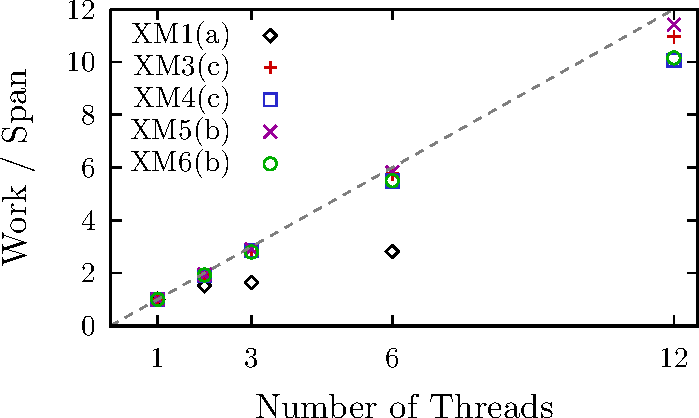
\includegraphics[width=.98\linewidth]{basex/exp_results/load_balance.pdf}
  \caption{Load balance}
  \label{fig:load-balance}
 \end{minipage}
 \hfill
 \begin{minipage}{.48\linewidth}
  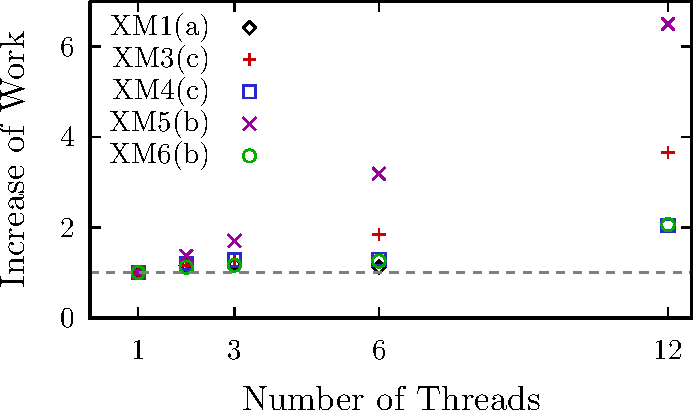
\includegraphics[width=.98\linewidth]{basex/exp_results/increase_of_work.pdf}
  \caption{Increase of work}
  \label{fig:increase-of-work}
 \end{minipage}
\end{figure}

% --------------------------------------------------
\subsection{Evaluation on Implementation of Query Partitioning Strategy}
\label{sec:qpseval}

Table~\ref{tab:qpstotaltime} summarizes the total execution time of the queries.
The ``orig \t{o}'' column shows the time for executing original queries XM1--XM6
and DBLP1--DBLP2 with BaseX's \texttt{xquery} command. The ``seq \t{s}'' columns
show the time for executing all the subquery one by one with a single thread.
The ``par \t{p}'' columns show  the time for executing the x query with one
thread and the with 12 or 6 threads depending on queries. The table also
includes reference of the speedup of parallel queries with respect to original
queries and the size of results of the original queries.


\begin{table}[t]
\centering
\caption{Summary of total execution times(ms) of queries by query partitioning}
\label{tab:qpstotaltime}
	\begin{tabular}{c|c|c|c|c|c}
		\hline
		\multirow{2}{*}{Key} & \multirow{2}{*}{orig \t{o}}  & \multicolumn{3}{c|}{Implementation of Query Partitioning} & Result size             \\ \cline{3-6}
		&                           & seq \t{s}             & par \t{p}             & \t{o}/\t{p}          & Final                   \\ \hline
		XM1(d)               & \multirow{2}{*}{25796.64} & 25326.472           & 11624.09           & 2.22           & \multirow{2}{*}{994M}   \\ \cline{1-1} \cline{3-5}
		XM1(e)               &                           & 31561.45            & 11514.87           & 2.24           &                         \\ \hline
		XM2(d)               & \multirow{2}{*}{1.33}     & 362.564             & 415.38             & 0.00           & \multirow{2}{*}{1.55 K} \\ \cline{1-1} \cline{3-5}
		XM2(e)               &                           & 4.05                & 1.26               & 1.06           &                         \\ \hline
		XM3(d)               & 595.75                    & 754.439             & 146.64             & 4.06           & 14.5 M                  \\ \hline
		XM4(d)               & \multirow{2}{*}{798.16}   & 1098.432            & 516.98             & 1.54           & \multirow{2}{*}{26.4 M} \\ \cline{1-1} \cline{3-5}
		XM4(e)               &                           & 1163.919            & 523.62             & 1.52           &                         \\ \hline
		XM5(d)               & \multirow{2}{*}{659.76}   & 869.089             & 288.21             & 2.29           & \multirow{2}{*}{15.9 M} \\ \cline{1-1} \cline{3-5}
		XM5(e)               &                           & 1536.161            & 1031.46            & 0.64           &                         \\ \hline
		XM6(d)               & \multirow{2}{*}{790.99}   & 744.873             & 646.67             & 1.22           & \multirow{2}{*}{22.2 M} \\ \cline{1-1} \cline{3-5}
		XM6(e)               &                           & 739.449             & 640.57             & 1.23           &                         \\ \hline
		DBLP1                & 3797.36                   & 6572.87             & 1618.51            & 2.35           & 133 M                   \\ \hline
    DBLP2                & 9684.71                   & 12524.70            & 6160.54            & 1.57           & 356 M                   \\ \hline
	\end{tabular}
    \vspace{10px}
	\centering
\caption{Breakdown of execution time (ms)}
\label{tab:qpsbreakdown}
\begin{tabular}{c|c|c|c|c|c|c|c}
	\hline
	\multirow{2}{*}{Key} & \multicolumn{6}{c|}{Subqueries}                              & \multirow{2}{*}{Merge} \\ \cline{2-7}
	& P=1      & P=2      & P=3      & P=6      & P=12    & t$^1$/t$^{12}$ &                        \\ \hline
	XM1(d)               & 25606.42 & 18583.66 & 18701.76 & 11420.36 &         & 2.24   & 203.73                 \\ \hline
	XM2(d)               & 356.67   & 384.08   & 367.99   & 345.89   & 415.38  & 0.86   & 0.00                   \\ \hline
	XM3(d)               & 540.14   & 327.03   & 241.33   & 159.63   & 141.82  & 3.81   & 4.82                   \\ \hline
	XM4(d)               & 897.38   & 786.46   & 550.56   & 507.15   &         & 1.77   & 9.83                   \\ \hline
	XM5(d)               & 670.15   & 415.35   & 314.01   & 284.40   & 282.14  & 2.38   & 6.07                   \\ \hline
	XM5(e)               & 701.94   & 698.77   & 735.18   & 828.65   & 1025.09 & 0.68   & 6.37                   \\ \hline
	XM6(d)               & 789.65   & 799.93   & 790.82   & 636.41   &         & 1.24   & 10.26                  \\ \hline
	DBLP1(d)             & 4035.83  & 2609.61  & 1931.22  & 1567.33  & 1584.97 & 2.55   & 33.53                  \\ \hline
\end{tabular}
\end{table}


\subsubsection{Total Execution Times and Speedups}

From Table~\ref{tab:qpstotaltime}, we can see that for most of the queries we
have obtained speedups of factors  more than 1 and XM3(d) obtains the most
speedup of a factor of 4.06. This means that we can accelerate the execution by
query partitioning for these queries. We also notice that there are two queries,
on the contrary, which have been decelerated: XM2(d) and XM5(e), even with up to
12 threads.

Now, we explain the causes of the slowdown of the two queries.

For XM2(d), one obvious reason is that the original query takes too short time
(only 1.33 ms), while the partitioned  subqueries take extra time for parallel
execution and merge operation. However, there still a big gap between XM2(d) and
XM2(e), i.e. XM2(e) takes quite less time than XM2(d) and is much close to the
original query of XM2. The difference is caused by the subqueries. For XM2(d),
since XM2 is partitioned by the \texttt{position} function at the position right
after \texttt{/site/regions/*}, it evaluates all the nodes that matches queries,
thus taking over 500 ms to complete the query. While for XM2(e), it actually
uses the attribute optimization so that the execution time has been greatly
reduced. This is because the subqueries of XM2(e) have complete paths. For
example, one of its subquery is
\texttt{/site/regions/africa/item/../parent::item/@id}. Since the full path is
contained in the subquires, BaseX can use \texttt{db:attribute("xmark10",
"category52")} to visit only the attribute nodes with the name ``\texttt{category52}'',
avoiding all redundant evaluations over nodes that are not of that attribute
name and thus achieving good optimization on execution time.

As for XM5(e), the partitioning point is just after the step of \texttt{bidder},
of which there are 597797 children nodes. For example, the first subquery of
XM5(e) is\\ \verb|/site/../bidder[position()= 1 to 49816]/increase|, letting P =
12. Note that the number of nodes that matches
\verb|/site/open_auctions/open_auction| is not 1 but 120000. In this case,
when BaseX evaluates the first subquery,  it actually traverses all 12000
\texttt{open\_auction} nodes and evaluates the first 69816 child nodes
\texttt{bidder} of each \texttt{open\_auction}. We investigate the number of
children of \texttt{open\_auction} and the max number is only 62. This means
that only the first subquery can retrieve resultant nodes, while the rest nodes
simply obtain nothing. From this result, we observe that to utilize
position-based query partitioning strategy, we need to guarantee the query before the
point where partition occurs should be a single path, i.e. the number of nodes that match
the query should be one.




\subsubsection{Breakdown of Execution Time}

In this section, we investigate execution times in greater details by analysing
the breakdown of execution time. All the settings are the same as that of data
partitioning.

We first observe that for most queries we can reduce execution time by adding
more threads. For example, XM1(d), XM3(d), XM4(d) and XM5(d) can be apparently
accelerated. While for XM2(d), and XM5(e), the execution times are actually
increased. Besides the reason given in the previous section, there is another
reason introduced in Section~\ref{sec:dpsscal} that the parallelization also
brings overhead compared to the original query and it increases with respect to
the number of threads increased. We also notice that XM6(d) is improved rather
small. This is because the imbalance of the input XML document
\texttt{xmark10.xml},  i.e. the six children of the root contain quite different
amount of descendant nodes,  thus making the reduction of execution time by
adding threads not very obvious.


\section{Observations and Perspectives}
\label{sect:concl}

In this paper, we have revived data partitioning \cite{BoLS09}
on top of BaseX and experimentally demonstrated, in the best case of non-trivial
queries, 4-fold speedup on a 12-core server. In this section, as
concluding remarks, we discuss possible improvement of BaseX in terms of 
partitioning strategies and further perspectives on BaseX.


\subsection{BaseX Extensions Desirable}

Since the implementations of query partitioning is reletively simple and mainly
influenced by the structure of input XML documents as we observed, we mainly
focus on the implementations of data partitioning strategies in this discussion.

Although the client-side implementation generally fell behind the server-side
one in our experiments, it has an advantage that it requires less functionality
of XML database servers. If that performance gap were filled, the client-side
one would be preferable. Since the performance gaps in prefix queries were small
even when their result sizes were more than 1 MB, the difference of cost between
sending prefix results to (local) clients and storing them in a server was
marginal. The dominant factor was the cost of sending prefix results back in the
form of long suffix queries and parsing them on a server.  A promising approach
to reducing this overhead is client-server streaming of the starting nodes of a
suffix query. Since one suffix query is in common applied to many starting
nodes, if the suffix query is given to a server in advance, the server can apply
it successively to incoming starting nodes and stream out results to clients.
With this streaming functionality additionally, the client-side implementation
would perform fast nearly to the server-side one.

There is also room for improvement of the server-side implementation. We store
block-partitioned arrays into an in-memory database as text parts and then
deserialize them to sequences. This is, to the best of our knowledge, the most
efficient way of preserving arrays on top of the current BaseX server, but is
merely a workaround because its serialization/deserialization is redundant. The
most efficient way is obviously to keep XQuery data structures as they are on
top of a server. We consider that it would not necessitate a drastic change of
BaseX. Only demand-driven serialization and new function \Src{deserialize}
suffice for it as follows. When XQuery values are put into a text part of an
in-memory database, they are not serialized immediately but keep their
representations. They will be serialized for a query just before the query tries
to read the text part. If a query applies \Src{deserialize} to the text part, it
returns their original representations in zero cost. It is worth noting that
because in-memory databases in BaseX will never be stored on disks,
demand-driven serialization per se is worth implementing to avoid serialization
into text parts not to be accessed.

\subsection{Further Perspectives}

Both data partitioning and index-based optimizations have worked together well
only with the simple way described in Section~\ref{sect:opt}. Both lie in the
same spectrum in the sense that performance gain is contingent on the statistics
of a given document. In fact, document statistics are known to be useful for
data partitioning (as well as query partitioning)
\cite{Bord10}. Statistics maintained together with indices
in BaseX should therefore be utilized for data partitioning together with
index-based optimizations. If we implement data partitioning into BaseX, a close
integration with both would be naturally feasible. Besides, statistics will be
available even outside BaseX by using \emph{probing} queries that count nodes
hitting at a specific step. The cost of several probing queries in advance to
data partitioning would matter little because simple counting queries are quite
fast on BaseX.  By using node counts, we can avoid the situation of an
insufficient number of prefix query results found in XM1(a). It will be a
lightweight choice in the sense of preserving a black-box use of BaseX.

It is challenging yet promising to extend data partitioning to distributed
databases with BaseX. The top part of a document to be traversed by prefix
queries can be either centralized or replicated. Bottom parts to be traversed by
suffix queries should be distributed as separate XML databases. Because the
whole database forms a simple collection of XML documents, horizontal
fragmentation \cite{kling11:dist_xml} will be well-suited but it can incur
imbalance in size among fragments. Balanced-size cheap fragmentation based on
partial trees \cite{HaMa16} will be promising for the complement to it. Existing
work \cite{DaGK14} on querying large integrated data will be relevant. Hybrid
partitioning \cite{BoLS09}, which is combination of data partitioning and query
partitioning, would become important because query partitioning requires
synchronization only in merging partial results and the number of
synchronizations matters more in distributed databases. Fragmentation-aware
hybrid partitioning is worth investigating. The most challenging part is to
implement integration with existing index-based optimizations so as to take
account of global information, where our idea described in
Section~\ref{sect:opt} will be useful but would not be trivially applicable.

\section{Summary}

First, as concluded in~\cite{BoLS09}, it is not obvious if data or query
partitioning would be beneficial. In our implementations, these are caused by
different factors. For the implementations of data partitioning, we need to
process a prefix query before processing the suffix queries in parallel. This is
a extra cost compared to the original query and the amout of extra time for
processing a prefix query relates to the result size of the prefix query. In
case the result size is large, it takes a lot time, such as DBLP1(a) and
DBLP2(a). While for the implementations of query parititioning, the imbalance of
XML documents have a dramatic influence on the query perfomrance and the
speedup.

Second, BaseX optimizer plays an important role in the reduction of execution
time. In case when BaseX optimizer is available, execution time can be greately
reduced. A very important feature of the optimizer is that it can also be
applied in parallel evaluation. Therefore, it is worth taking the optimizations
to reduce the execute time as long as the partition of subqueries can meet the
conditions of the BaseX optimizer.

Third, the experiment results clearly show that we can achrive speedup up to 4,
which have strongly proved that the partitioning stragegies are available not
only on XML trees but also on XML database engines. However, the availability of
these stragegies is significantly dependent on the implementations and the XML
database engine/processor. Properly combined with the features of the XML
database engine/processor used for implementation, we can achrive significant
performance improvements over the original strategies, such as the server-side
implementation of data partitioning strategy.

